\documentclass[12pt,letterpaper]{article}

\usepackage[spanish,es-tabla,es-nodecimaldot]{babel}
\usepackage{amsmath}
\usepackage[utf8]{inputenc}
\usepackage[T1]{fontenc}
\usepackage{lmodern}
\usepackage{graphicx}
\usepackage{listings}
\usepackage{anysize} 
\usepackage{fancyhdr}
\usepackage{amsmath}
\usepackage{pdfpages}
\usepackage{graphics}
\usepackage{capt-of}
\usepackage{tabularx}
\usepackage[colorlinks=true,plainpages=true,citecolor=blue,linkcolor=blue]{hyperref}

\marginsize{2cm}{2cm}{2cm}{2cm}
\pagestyle{fancy}
\fancyhf{Redes de Telecomunicaciones}
\fancyhead[L]{\footnotesize UPIITA-IPN} 
\fancyhead[R]{\footnotesize 4TV2} 
\fancyfoot[R]{\footnotesize Memoría técnica}
\fancyfoot[C]{\thepage}
\fancyfoot[L]{\footnotesize La Costeña} 

\renewcommand{\footrulewidth}{0.4pt}
\renewcommand{\spanishtablename}{Tabla}
\renewcommand{\labelitemii}{$\star$}

\begin{document}

\includepdf[pages={1}]{portada2}

\newpage
\tableofcontents
\listoffigures
\listoftables

\newpage
\section{Poligonal}

\newpage
\section{Ruta}
\subsection{Ruta principal y alternativa}
Ruta principal tomando la mayor parte del trayecto por metro.
\begin{figure}[ht]
    \centering
    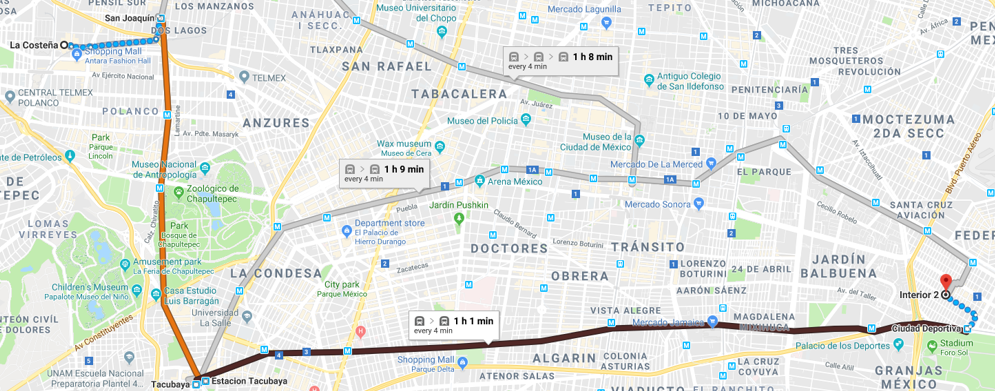
\includegraphics[width=.9\textwidth]{f2.png}
    \caption{Ruta principala a escala.}
\end{figure}

La ruta alternativa cuenta con tramo principal por avenidas 
vehiculares.
\begin{figure}[ht]
    \centering
    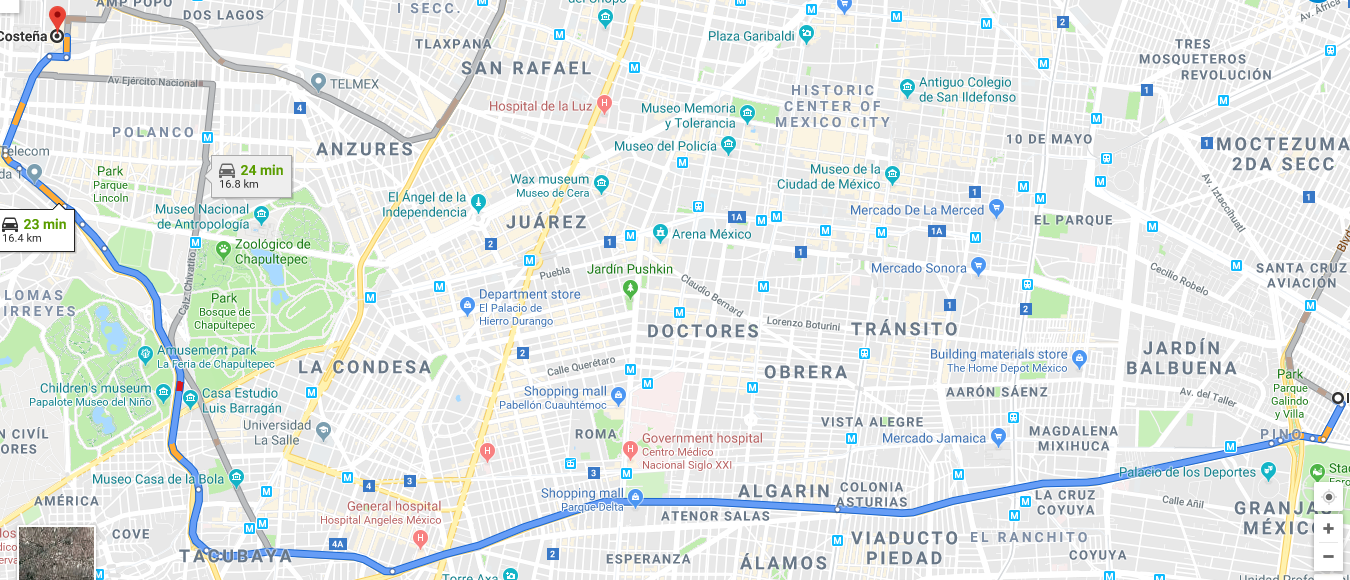
\includegraphics[width=.9\textwidth]{f3.png}
    \caption{Ruta alternativa a escala.}
\end{figure}

\newpage
\subsection{Salida de corporativo}
Se propone que la salida de la salida de la fibra sea por el 
sótano que es donde se encuentra el site del edificio.
\begin{figure}[ht]
    \centering
    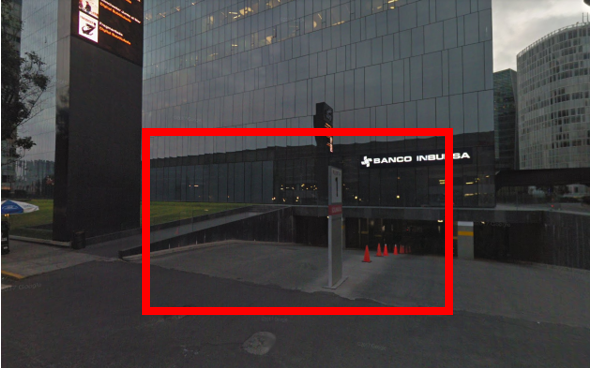
\includegraphics[width=.6\textwidth]{f0.png}
    \caption{Salida de corporativo.}
\end{figure}

Una vez fuera se tomará el siguiente registro para llevarlo por 
subsuelo hasta el metro.
\begin{figure}[ht]
    \centering
    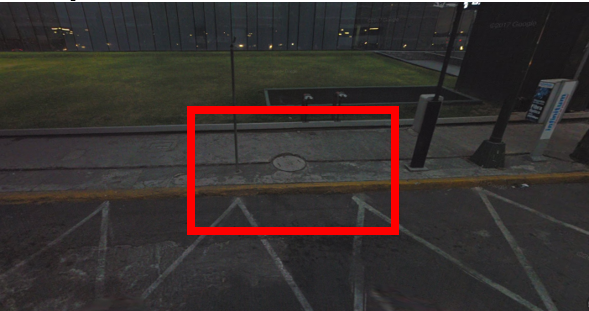
\includegraphics[width=.7\textwidth]{f1.png}
    \caption{Registro donde iniciar el recorrido.}
\end{figure}

\newpage
\subsection{Puntos críticos: Ruta principal}
\subsubsection{Primer tramo}
A continuación se muestra el primer tramo del recorrido. Este 
tramo es del corporativo al metro.
\begin{figure}[ht]
    \centering
    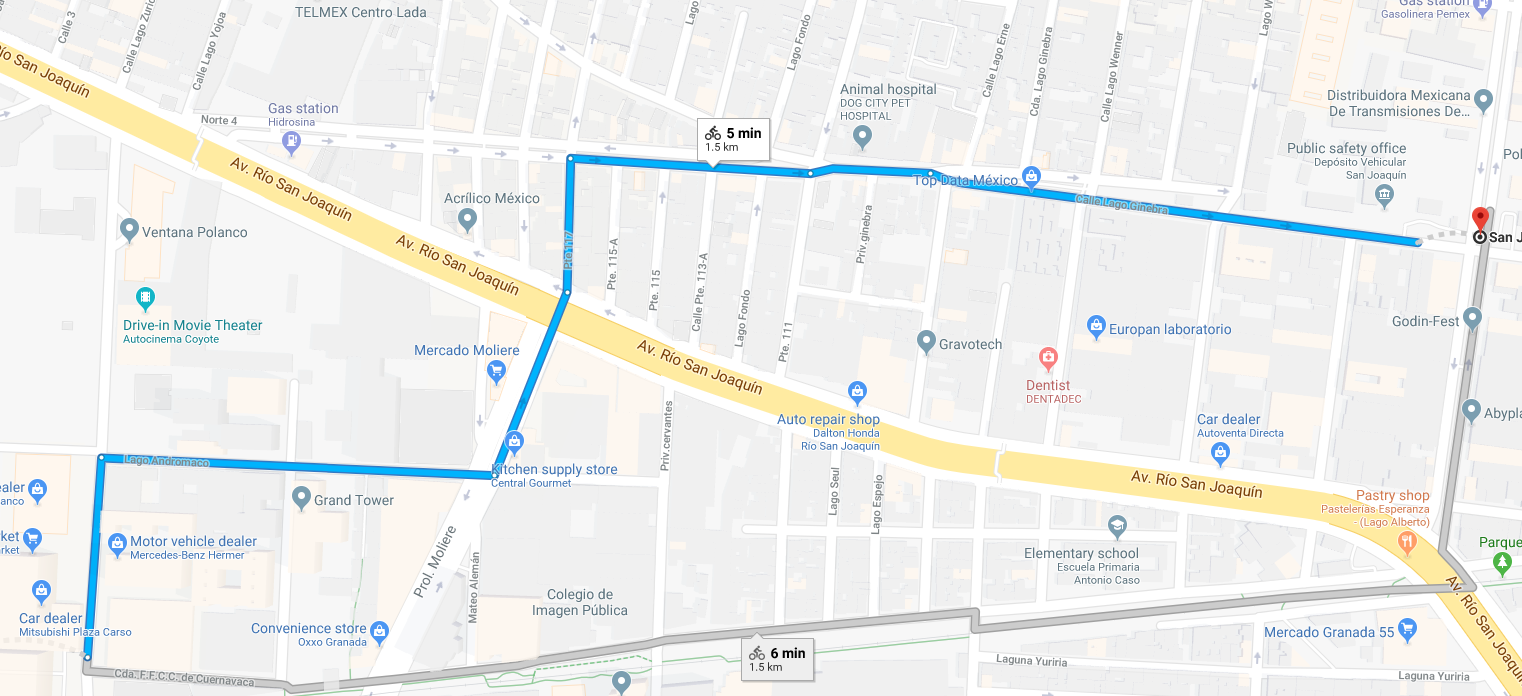
\includegraphics[width=.8\textwidth]{f5.png}
    \caption{Vista aerea primer tramo.}
\end{figure}

El primer punto crítico se encuentra en el puente para cruzar la 
avenida Río San Joaquín.
\begin{figure}[ht]
    \centering
    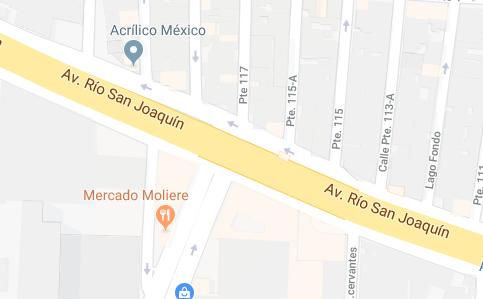
\includegraphics[width=.6\textwidth]{f4.png}
    \caption{Vista aerea punto crítico.}
\end{figure}

Para sortear este obstáculo se tendrá que utilizar un tendido aéreo 
para posteriormente volver a introducirlo en el subsuelo.
\begin{figure}[ht]
    \centering
    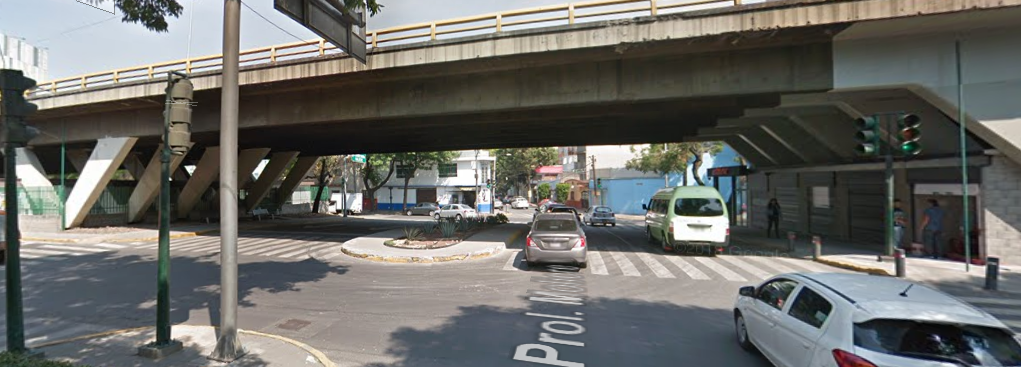
\includegraphics[width=1\textwidth]{f6.png}
    \caption{Punto crítico.}
\end{figure}

\subsubsection{Segundo tramo}
El segundo tramo consta de todo el recorrido en metro. En este 
tramo se cuenta con un punto crítico es cúal es el cambio de lineas 
9 y 4.
\begin{figure}[ht]
    \centering
    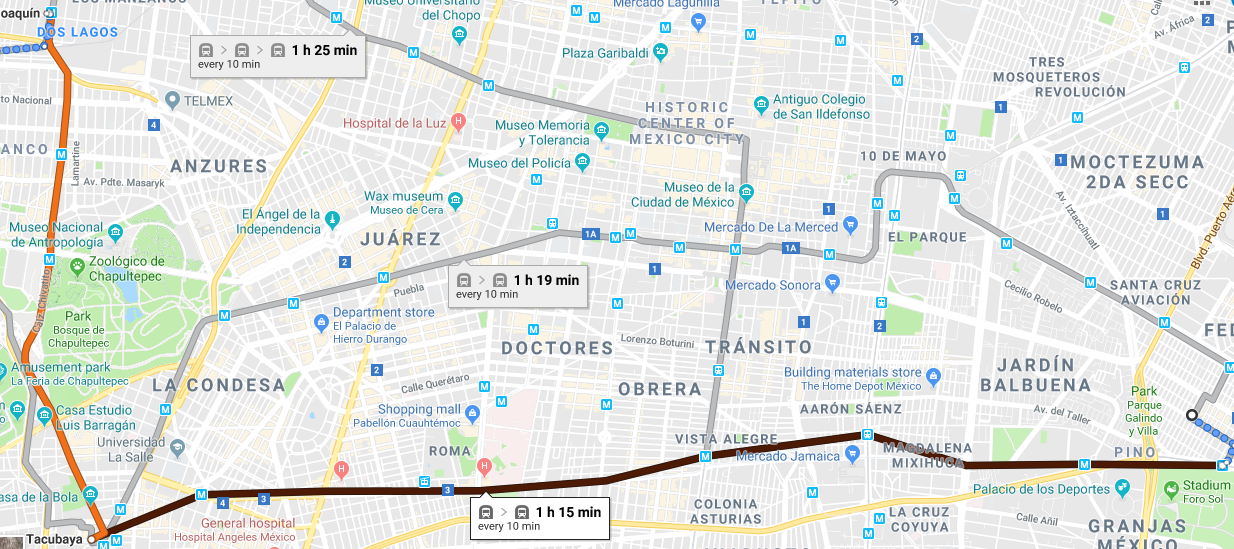
\includegraphics[width=1\textwidth]{f7.png}
    \caption{Vista aerea segundo tramo.}
\end{figure}
\\
El punto crítico de este tramo se encuentra en el cambio de lineas.
\begin{figure}[ht]
    \centering
    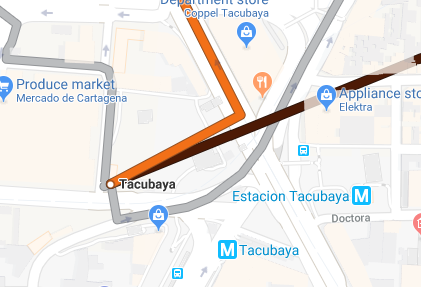
\includegraphics[width=.5\textwidth]{f8.png}
    \caption{Punto crítico segundo tramo.}
\end{figure}

\newpage
\subsubsection{Tercer tramo}
El tercer tramo del recorrido consta de la salida del metro hasta
el centro de datos.
\begin{figure}[ht]
    \centering
    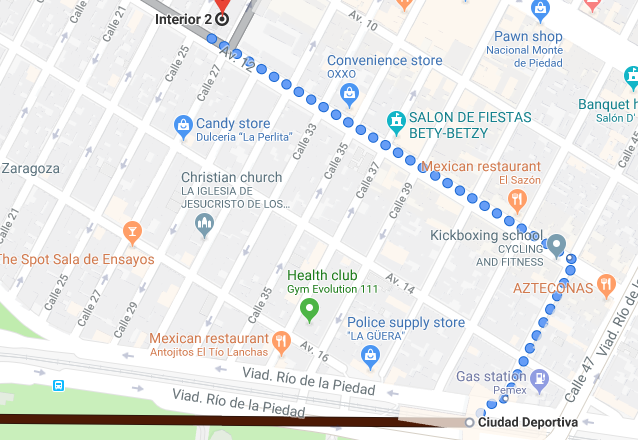
\includegraphics[width=.5\textwidth]{f9.png}
    \caption{Punto crítico segundo tramo.}
\end{figure}

En este tramo el punto crítico se encuentra a la salida del metro 
para mandarlo hacía el corporativo por tendido aéreo.
\begin{figure}[ht]
    \centering
    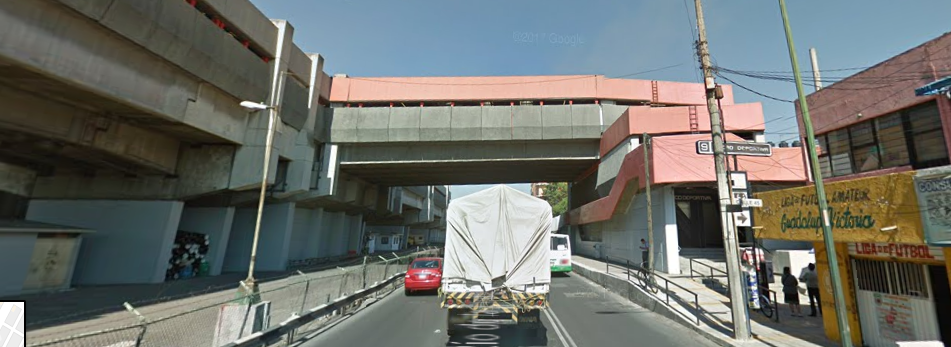
\includegraphics[width=.9\textwidth]{f10.png}
    \caption{Punto crítico segundo tramo.}
\end{figure}

\newpage
\subsection{Estemación}

\newpage
\section{Ductos}

\newpage
\section{Fibras}

\newpage
\section{Arquitectura}

\newpage
\section{E-commerce}


\newpage
\begin{thebibliography}{20}
    \bibitem{anchobanda}
    IEEE Standard Definitions of Terms for Antennas, in IEEE Std 145-1993 , vol., no., pp.1-32, 18 July 1993

    \bibitem{radiacion}
    Constantine A. Balanis: Antenna Theory, Analysis and Design, John Wiley and Sons, Inc., 2nd ed. 1982.
    
    \bibitem{polarizacion}
    Constantine A. Balanis: Modern Antenna Handbook, Wiley, 2007.

    \bibitem{haz}
    W. L. Stutzman and G. A. Theile, Antenna theory and design. John Wiley and Sons, Inc., 1998.
\end{thebibliography}

\end{document}